\documentclass[a4paper]{article}

\usepackage{anyfontsize}
\usepackage{amsmath}

\usepackage[no-math]{fontspec}
\setmainfont{TeX Gyre Termes}
\usepackage{unicode-math}
\unimathsetup{bold-style=ISO,sans-style=italic}
\setmathfont{XITS Math}
\AtBeginDocument{
  \let\uglymathbf\mathbf
  \renewcommand\mathbf\symbf
  \let\uglymathsf\mathsf
  \renewcommand\mathsf\symsf
}

\AtBeginDocument{
  \let\uglyepsilon\epsilon
  \renewcommand\epsilon\varepsilon
}

\usepackage{bm}
\renewcommand\bm\symbf

\usepackage{indentfirst}
\setlength{\parindent}{0em}
\usepackage{autobreak}
\allowdisplaybreaks
\usepackage{parskip}
\usepackage{geometry}
\geometry{top=3cm,bottom=3cm,left=2cm,right=2cm}
\usepackage{tikz}

\usepackage[fontset=none]{ctex}
\setCJKmainfont{Adobe Song Std}[BoldFont=Noto Sans CJK SC Medium]

\begin{document}

\title{\textbf{实测天体物理作业}}
\author{1900011604\ \ 张植竣\ \ 北京大学}
\date{2022年2月28日}
\maketitle

\begin{enumerate}

    \item[1.]
    单位球面的总面积为：
    \[
        S = \iint\limits_\Omega \sin\theta\,\mathrm{d}\theta\mathrm{d}\varphi
    \]
    以球面度为单位时：
    \begin{align*}
        S
        &= \iint\limits_\Omega \sin\theta\,\mathrm{d}\theta\mathrm{d}\varphi \\
        &= \int_0^\pi \sin\theta\,\mathrm{d}\theta \int_0^{2\pi} \mathrm{d}\varphi \\
        &= (-\cos\theta)|_0^\pi \cdot \phi|_0^{2\pi} \\
        &= 4\pi\,\mathrm{sr}
    \end{align*}
    以平方度为单位时：
    \begin{align*}
        S
        &= \iint\limits_\Omega \sin\theta\,\mathrm{d}\theta\mathrm{d}\varphi \\
        &= \int_0^{180} \sin\theta\,\mathrm{d}\theta \int_0^{360} \mathrm{d}\varphi \\
        &= \left.\left(-\frac{180}{\pi}\cos\theta\right)\right|_0^{180} \cdot \phi|_0^{360} \\
        &= \frac{129600}{\pi}\,\mathrm{deg^2} \\
        &\approx 41253\,\mathrm{deg^2}
    \end{align*}
    可见有：
    \[
        1\,\mathrm{sr} = \frac{32400}{\pi^2}\,\mathrm{deg^2} = \left(\dfrac{180}{\pi}\right)^2\,\mathrm{deg^2} \approx 3282.8\,\mathrm{deg^2}
    \]
    由于观测分辨率为$1\,\mathrm{beam}=1\,\mathrm{arcmin^2}$，且$1\,\mathrm{deg^2}=60^2\,\mathrm{arcmin^2}=3600\,\mathrm{arcmin^2}$，故：
    \[
        1\,\mathrm{sr} = 3600\cdot\frac{129600}{\pi}\,\mathrm{beam} = 1.1818\times10^7\,\mathrm{beam}
    \]

    \bigskip
    \item[2.]
    设偶极天线的长度为$l$（$l\ll\lambda$），中心处最大电流为$I_0$，则沿天线上的电流分布近似为线性形式：
    \[
        I(z) = I_0(1-\frac{2}{l}|z|),\quad |z|\leqslant\frac{l}{2}
    \]
    \begin{center}
        \begin{tikzpicture}
            \draw[thick,->,>=latex] (0,0)--(0,2.5);
            \draw[thick,->,>=latex] (-4,0)--(4,0) node[right] {$z$};
            \draw (-3.5,0)--(0,1.5);
            \draw (3.5,0)--(0,1.5);
            \draw (-0.25,2.6) node {$I$};
            \draw (-0.25,1.7) node {$I_0$};
            \draw (-3.65,0.55) node {$-\dfrac{l}{2}$};
            \draw (3.5,0.55) node {$\dfrac{l}{2}$};
            \draw (-3.5,-0.3)--(-0.1,-0.3);
            \draw (3.5,-0.3)--(0.1,-0.3);
            \draw (-0.1,-0.8)--(-0.1,-0.3);
            \draw (0.1,-0.8)--(0.1,-0.3);
        \end{tikzpicture}
    \end{center}
    设天线的电偶极矩为$\bm{p}=p\mathrm{e}^{-i\omega t}\hat{z}$，则有：
    \[
        \frac{\partial p}{\partial t} = \iiint\limits_V J(x)\,\mathrm{d}V = \int_{-\tfrac{l}{2}}^{\tfrac{l}{2}} I(z)\,\mathrm{d}z = \frac{1}{2}I_0l,\quad
        \bm{p}=\frac{i}{2\omega}I_0l\mathrm{e}^{-i\omega t}\hat{z}
    \]
    其产生的辐射场为：
    \[
        \bm{E}
        = \frac{p\omega^2}{4\pi\epsilon_0c^2}\sin\theta\frac{\mathrm{e}^{ikr}}{r}\hat{\theta}
        = \frac{i\omega I_0l}{8\pi\epsilon_0c^2}\sin\theta\frac{\mathrm{e}^{-i(\omega t-kr)}}{r}\hat{\theta}
    \]
    \[
        \bm{H}
        = \frac{p\omega^2}{4\pi c}\sin\theta\frac{\mathrm{e}^{ikr}}{r}\hat{\phi}
        = \frac{i\omega I_0l}{8\pi c}\sin\theta\frac{\mathrm{e}^{-i(\omega t-kr)}}{r}\hat{\phi}
    \]
    则Poynting矢量为：
    \[
        \bm{S}
        = \frac{1}{2}\bm{E}\times\bm{H}^*
        = \frac{\mu_0c}{32}\left(\frac{I_0l}{r\lambda}\right)^2\sin^2\theta\hat{r}
    \]
    其功率的角分布可以从Poynting矢量得到：
    \[
        P_{\bm{n}}
        = \frac{\mathrm{d}P}{\mathrm{d}\Omega_{\bm{n}}}
        = \lim_{r\to\infty} \hat{r}\cdot(r^2\bm{S})
        = \frac{\mu_0c}{32}\left(\frac{I_0l}{\lambda}\right)^2\sin^2\theta
    \]
    则有：$P_{max}=\dfrac{\mu_0c}{32}\left(\dfrac{I_0l}{\lambda}\right)^2$，归一化的功率方向图$P_{\bm{n}}(\theta,\phi)=\sin^2\theta$，绘图如下：
    \begin{center}
        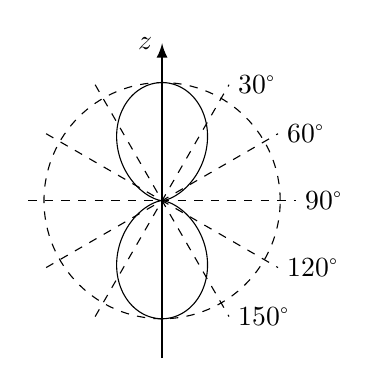
\begin{tikzpicture}
            \draw[thick,->,>=latex] (0,-2)--(0,2) node[left] {$z$};
            \draw[dashed] (-0.85,-1.4722432)--(0.85,1.4722432) node[right] {$30^\circ$};
            \draw[dashed] (-1.4722432,-0.85)--(1.4722432,0.85) node[right] {$60^\circ$};
            \draw[dashed] (-1.7,0)--(1.7,0) node[right] {$90^\circ$};
            \draw[dashed] (-1.4722432,0.85)--(1.4722432,-0.85) node[right] {$120^\circ$};
            \draw[dashed] (-0.85,1.4722432)--(0.85,-1.4722432) node[right] {$150^\circ$};
            \draw[dashed] (0,0) circle [radius=1.5];
            \draw[domain=0:360,samples=1000] plot (\x:{1.5*(sin(\x))^2});
        \end{tikzpicture}
    \end{center}
    天线的总功率为：
    \[
        P = \frac{\mu_0\pi c}{12}\left(\frac{I_0l}{\lambda}\right)^2
    \]
    方向增益为：
    \[
        G_{\bm{n}}(\theta,\phi) = \frac{4\pi P_{\bm{n}}}{P} = \frac{3}{2}\sin^2\theta
    \]
    方向系数$D=G_{max}=\dfrac{3}{2}$，以$\mathrm{dB}$为单位表示为：
    \[
        D_{\mathrm{dB}} = 10\lg\frac{3}{2} = 1.761\,\mathrm{dB}
    \]
    天线立体角为：
    \[
        \Omega_A = \frac{4\pi}{G_{max}} = \iint\limits_{S}P_{\bm{n}}\,\mathrm{d}\Omega = \frac{8\pi}{3}
    \]

    \bigskip
    \item[3.]
    流量密度为：
    \[
        S = \frac{P}{4\pi r^2\Delta\nu} = \frac{500\,\mathrm{W}}{4\pi\times(1\,\mathrm{m})^2\times1\,\mathrm{MHz}} = 3.979\times10^{-7}\,\mathrm{Wm^{-2}Hz^{-1}} = 3.979\times10^{19}\,\mathrm{Jy}
    \]

    \bigskip
    \item[4.]
    天线立体角为：
    \begin{align*}
        \Omega_A
        &= \iint\limits_{S}P_{\bm{n}}\,\mathrm{d}\Omega \\
        &= 0.1\times2\pi(1-\cos10^\circ) - 0.1\times2\pi(1-\cos1^\circ) + 1\times2\pi(1-\cos1^\circ) \\
        &= 1.04\times10^{-2}
    \end{align*}
    主瓣立体角为：
    \begin{align*}
        \Omega_\mathrm{MB}
        &= \iint\limits_\mathrm{MB}P_{\bm{n}}\,\mathrm{d}\Omega \\
        &= 1\times2\pi(1-\cos1^\circ) \\
        &= 9.57\times10^{-4}
    \end{align*}
    主瓣效率为：
    \[
        \eta_{B} = \frac{\Omega_\mathrm{MB}}{\Omega_A}\times100\% = 9.2\%
    \]

\end{enumerate}

\end{document}